\documentclass[main.tex]{subfiles}

\begin{document}

\section{Software Architecture}\label{sec:software-architecture}

The overall DApp consists of various components, summarized in figure \ref{fig:gethdomains_architecture}:
\begin{itemize}
    \item The code is stored in a GitHub repository, publicly accessible from the date of the submission of this project: each team member is set as a collaborator and has full access to it
    \item Every time a team member pushes his commits, a CI/CD pipeline on GitHub Actions will run, deploying the webapp and making the new version reachable from the associated website
    \item In addition to it, the HTML documentation of the latest Solidity smart contracts is generated and published (\href{https://gethdomains.best/smart_contract_docs.html}{https://gethdomains.best/smart\_contract\_docs.html})
    \item The webapp will interact with the code stored and running on the blockchain through a Web3 provider like Metamask
    \item The \texttt{DomainMarketplace} smart contract (which manages the domain names selling and registration) interacts with the Geth smart contract to manipulate the users' balance
    \item Currently, both smart contracts are running on Sepolia testnet (a semi-production environment), after being tested and developed using Truffle and Ganache
\end{itemize}
It's noticeable that no centralized backend exists, and that's the core of Decentralized Applications, like GethDomains.

\begin{figure}[htbp]
    \centering
    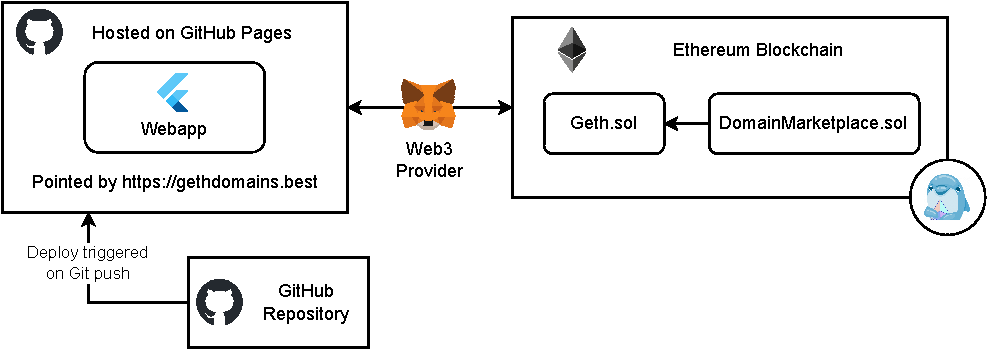
\includegraphics[width=\textwidth]{figures/gethdomains_architecture.pdf}
    \caption{GethDomains DApp general architecture}
    \label{fig:gethdomains_architecture}
\end{figure}
\newpage
\subsection{UML Sequence Diagram}
Sequence Diagrams are use to show intereactions between the entities of our Dapp. They show the interections in a time sequence exchange messages. Below there are the sequence diagrams of the most important operation in our Dapp.\\

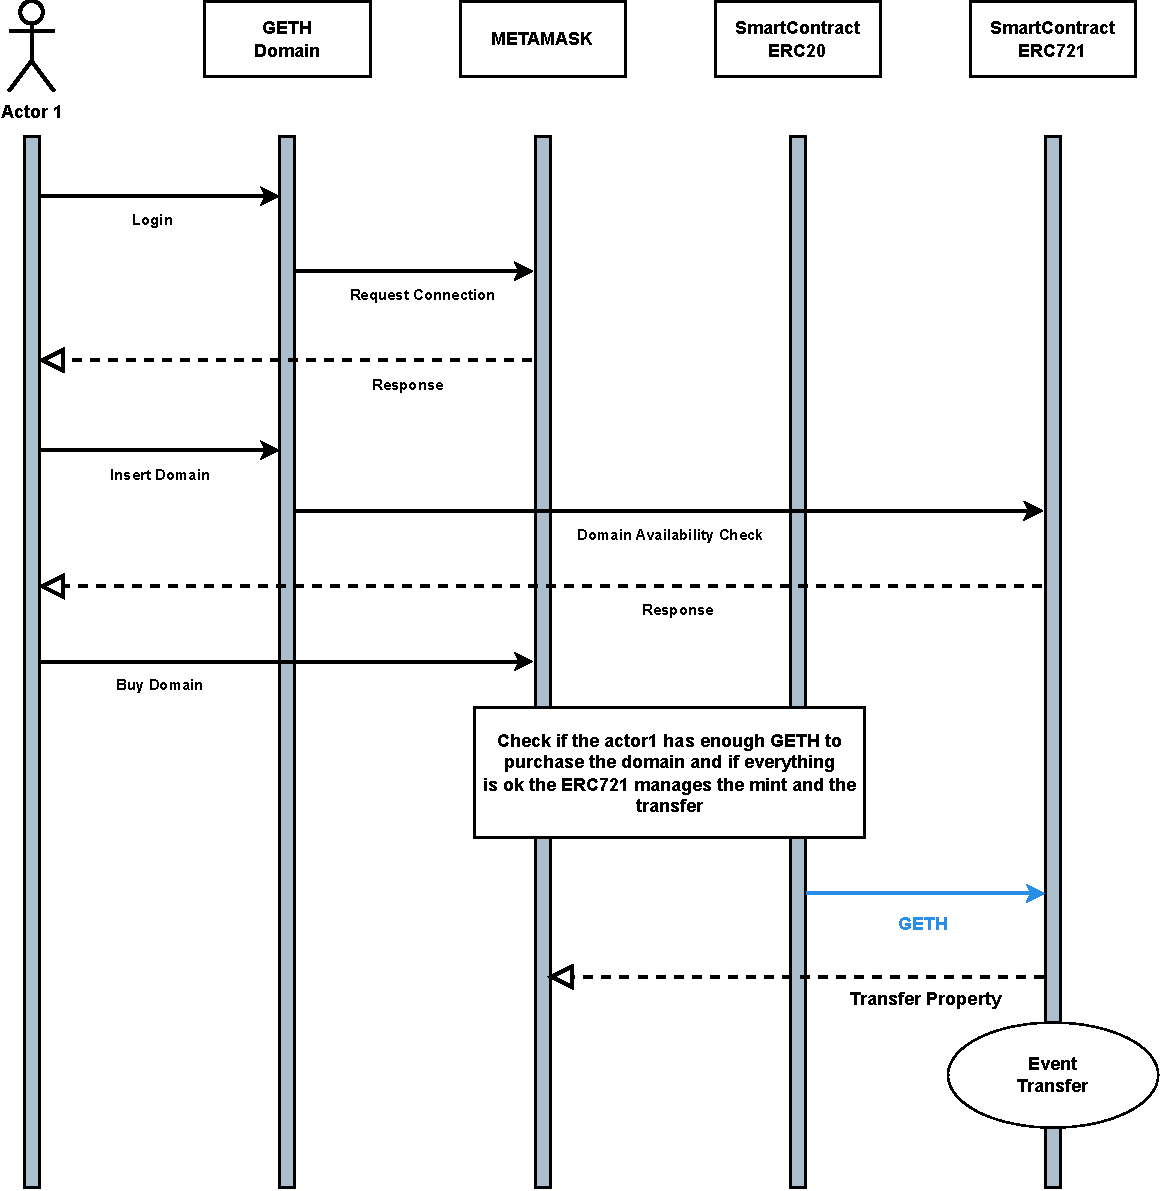
\includegraphics[width=0.7\linewidth]{figures/PurchaseNewDomain.pdf}\\
% \caption{Sequence diagram of the purchase of a domain}
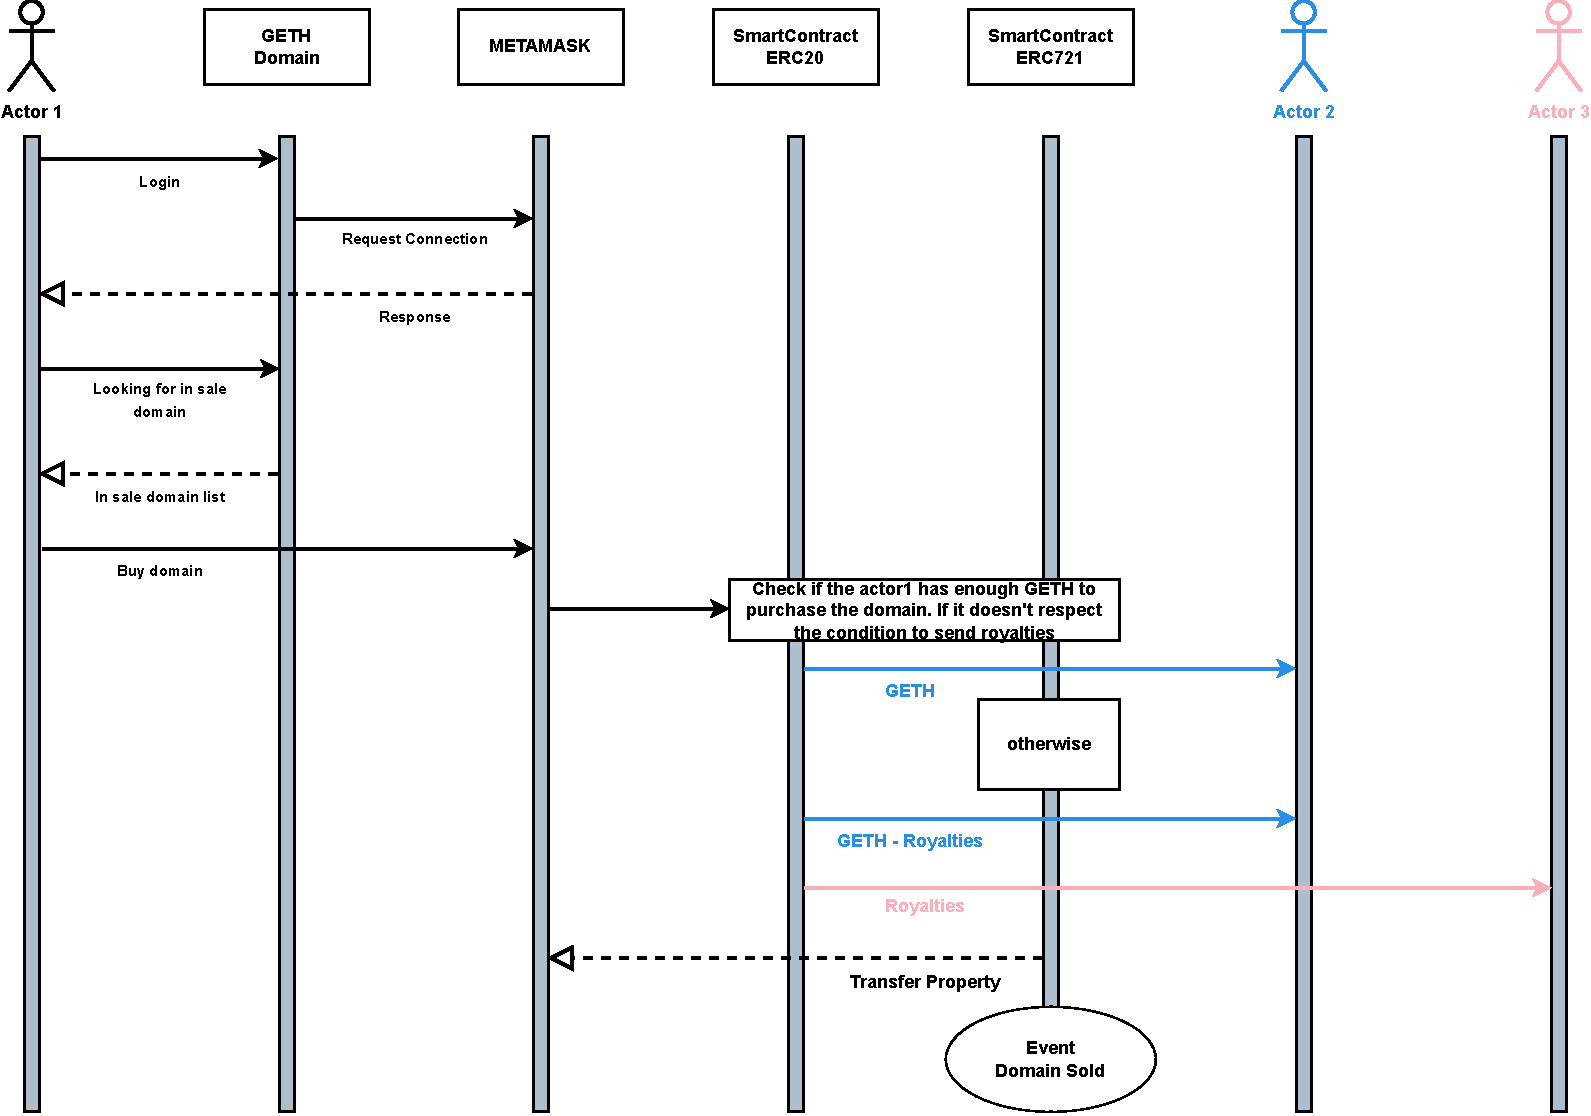
\includegraphics[width=0.8\linewidth]{figures/UnioneBuy.drawio.pdf}\\

% 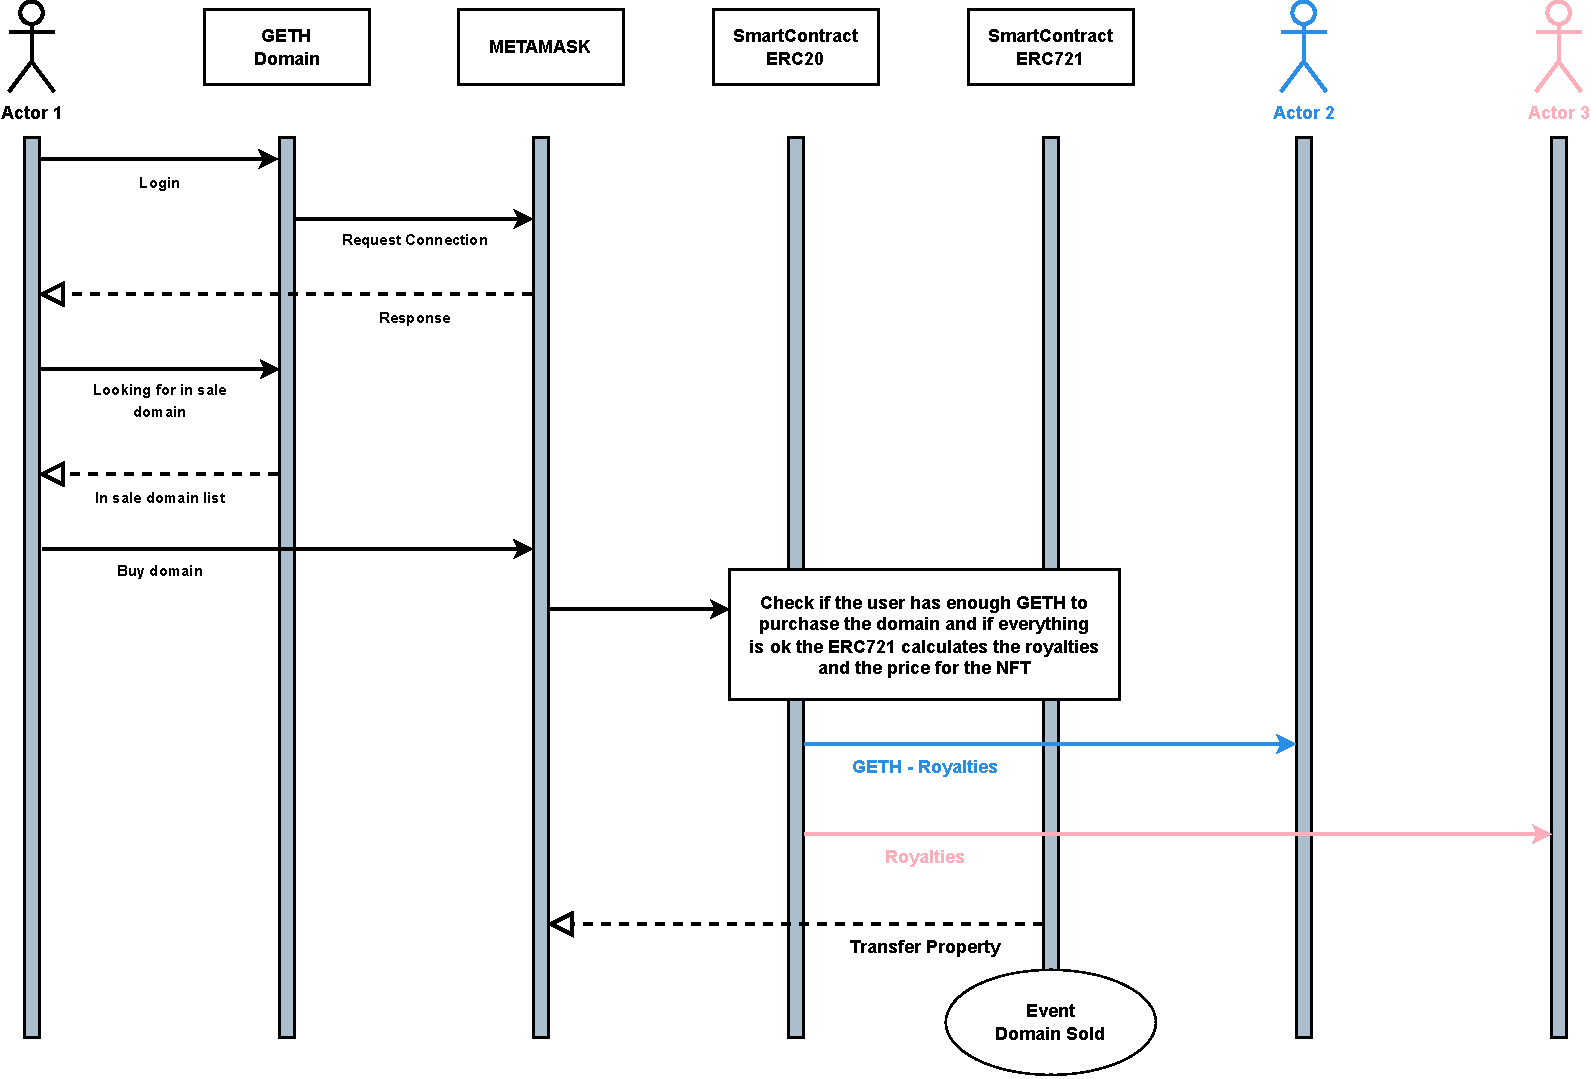
\includegraphics[width=1\linewidth]{figures/BuyWithRoyalties.drawio.pdf}\\

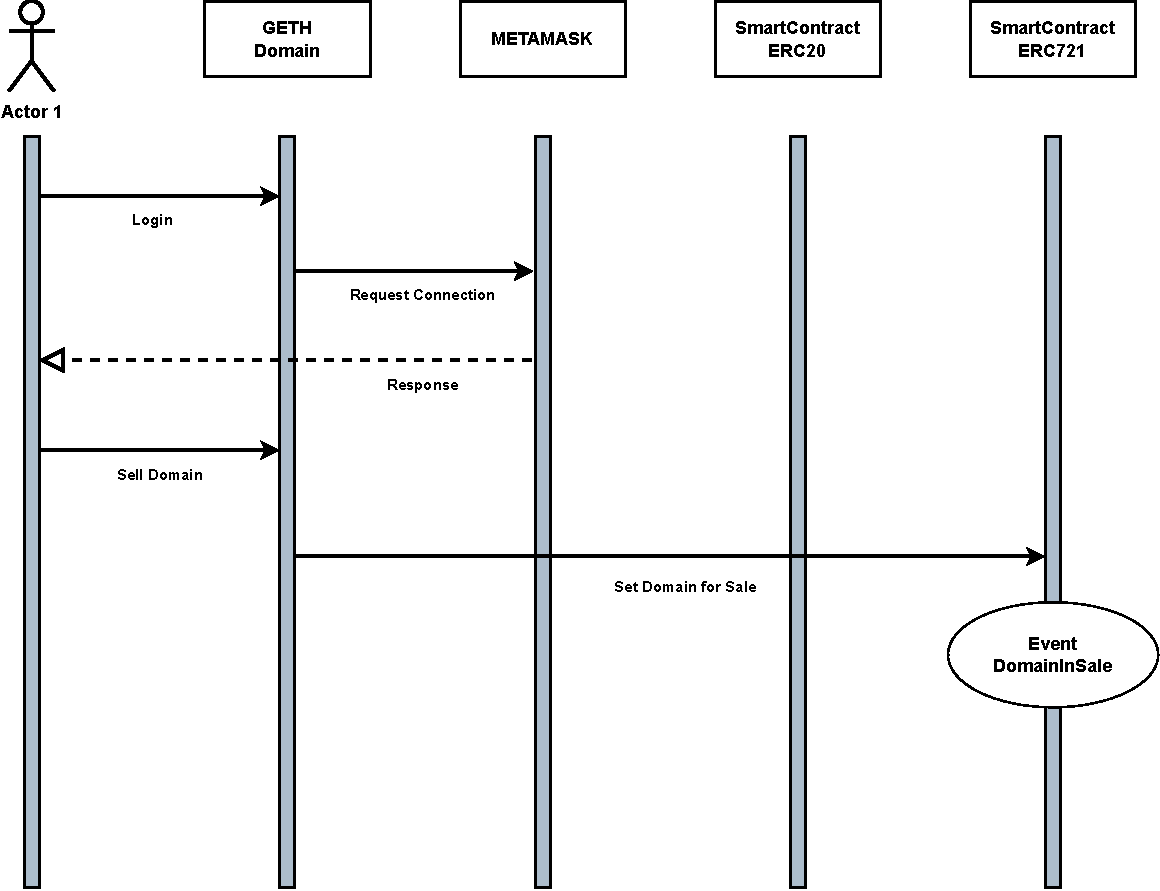
\includegraphics[width=0.8\linewidth]{figures/InSaleDomain.drawio.pdf}\\


% \subsection{UML Use Case Diagram}
% The Use case Diagram represents the system functionalities from the user's prospective. It's composed by actors and functionalities.
% In Our Dapp each user is a peer who is allowed to perform every action. 

% 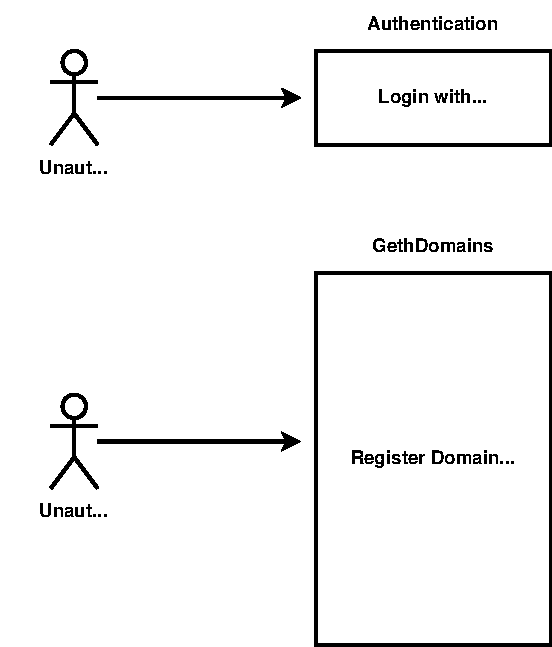
\includegraphics[scale=0.5]{figures/UseCase.drawio.pdf}

% \subsection{UML Activity Diagram}
% An Activity Diagram is used to model the dynamic aspects of a system, focusing on the workflow or activities performed within the system. Activity diagrams are particularly useful for visualizing the flow of activities, \textbf{actions}, and \textbf{decisions} in a process or use case.
\newpage
\subsection{UML Class Diagram}
A class diagram represents the static structure of a system by depicting the classes, their attributes, methods, and the relationships among classes. It provides a visual representation of the essential components and their \textbf{relationships} in the design or structure of a software system.

% 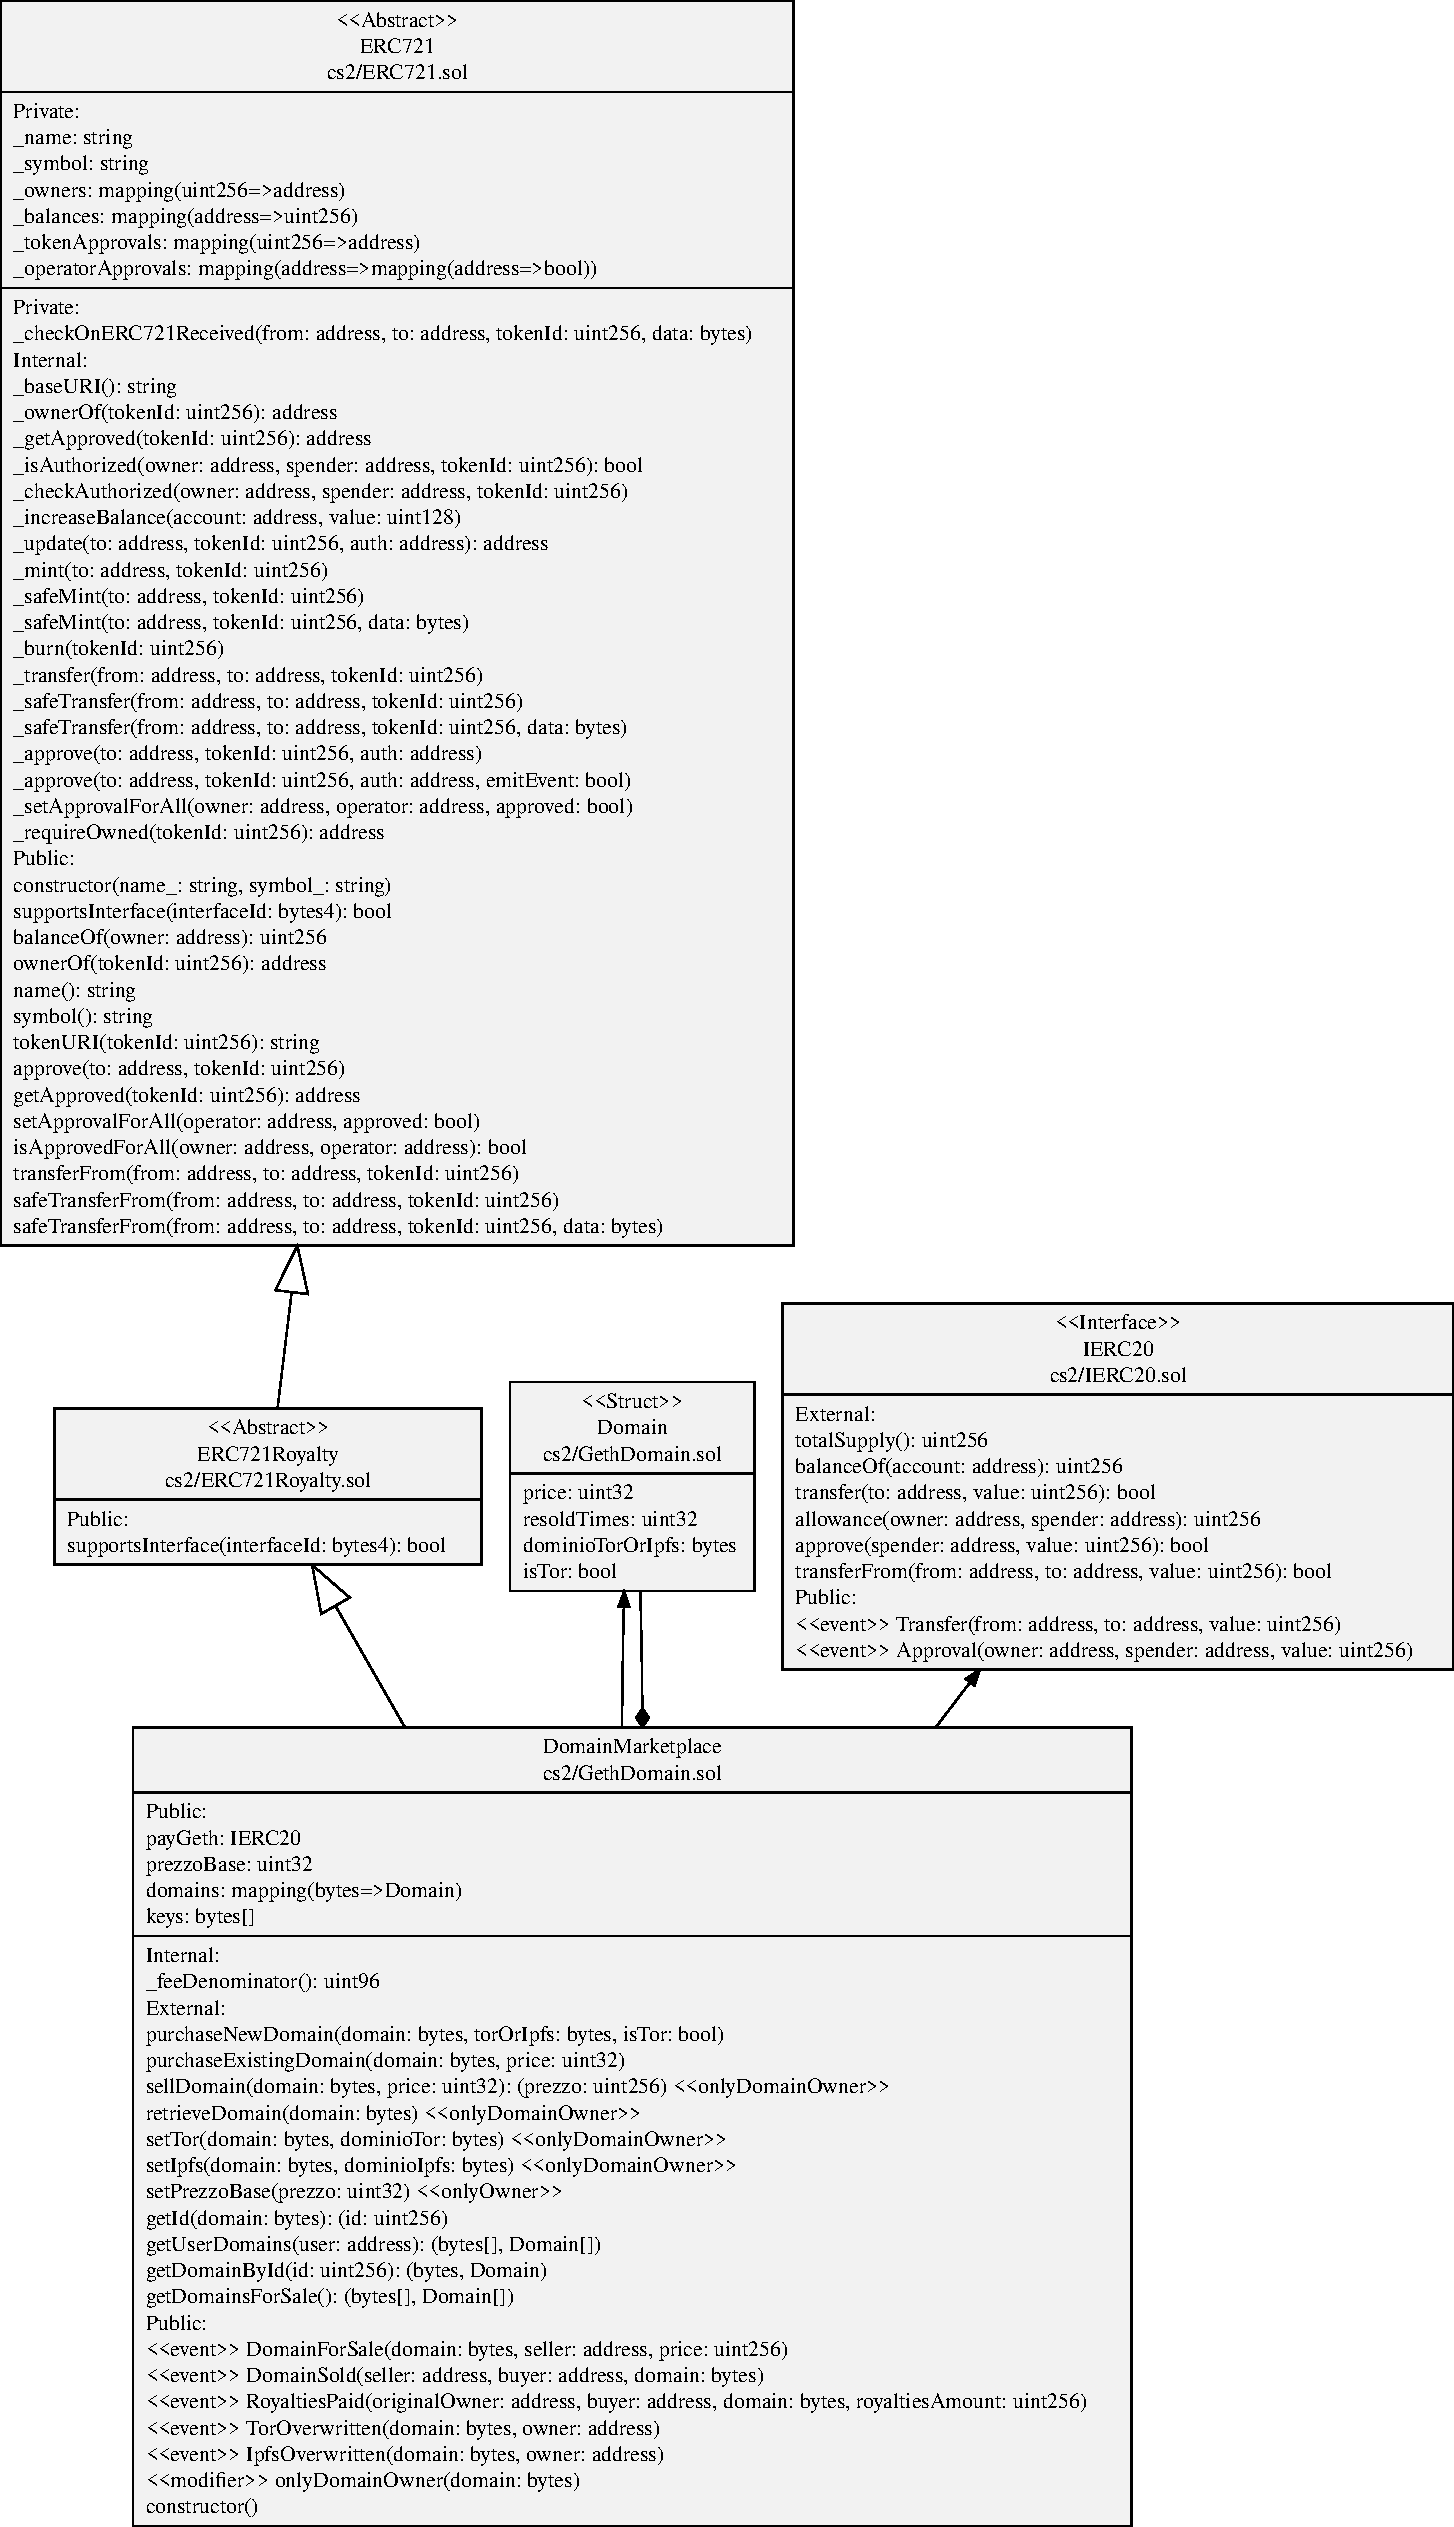
\includegraphics[scale=0.5]{figures/Market2-cropped.pdf}\\
% 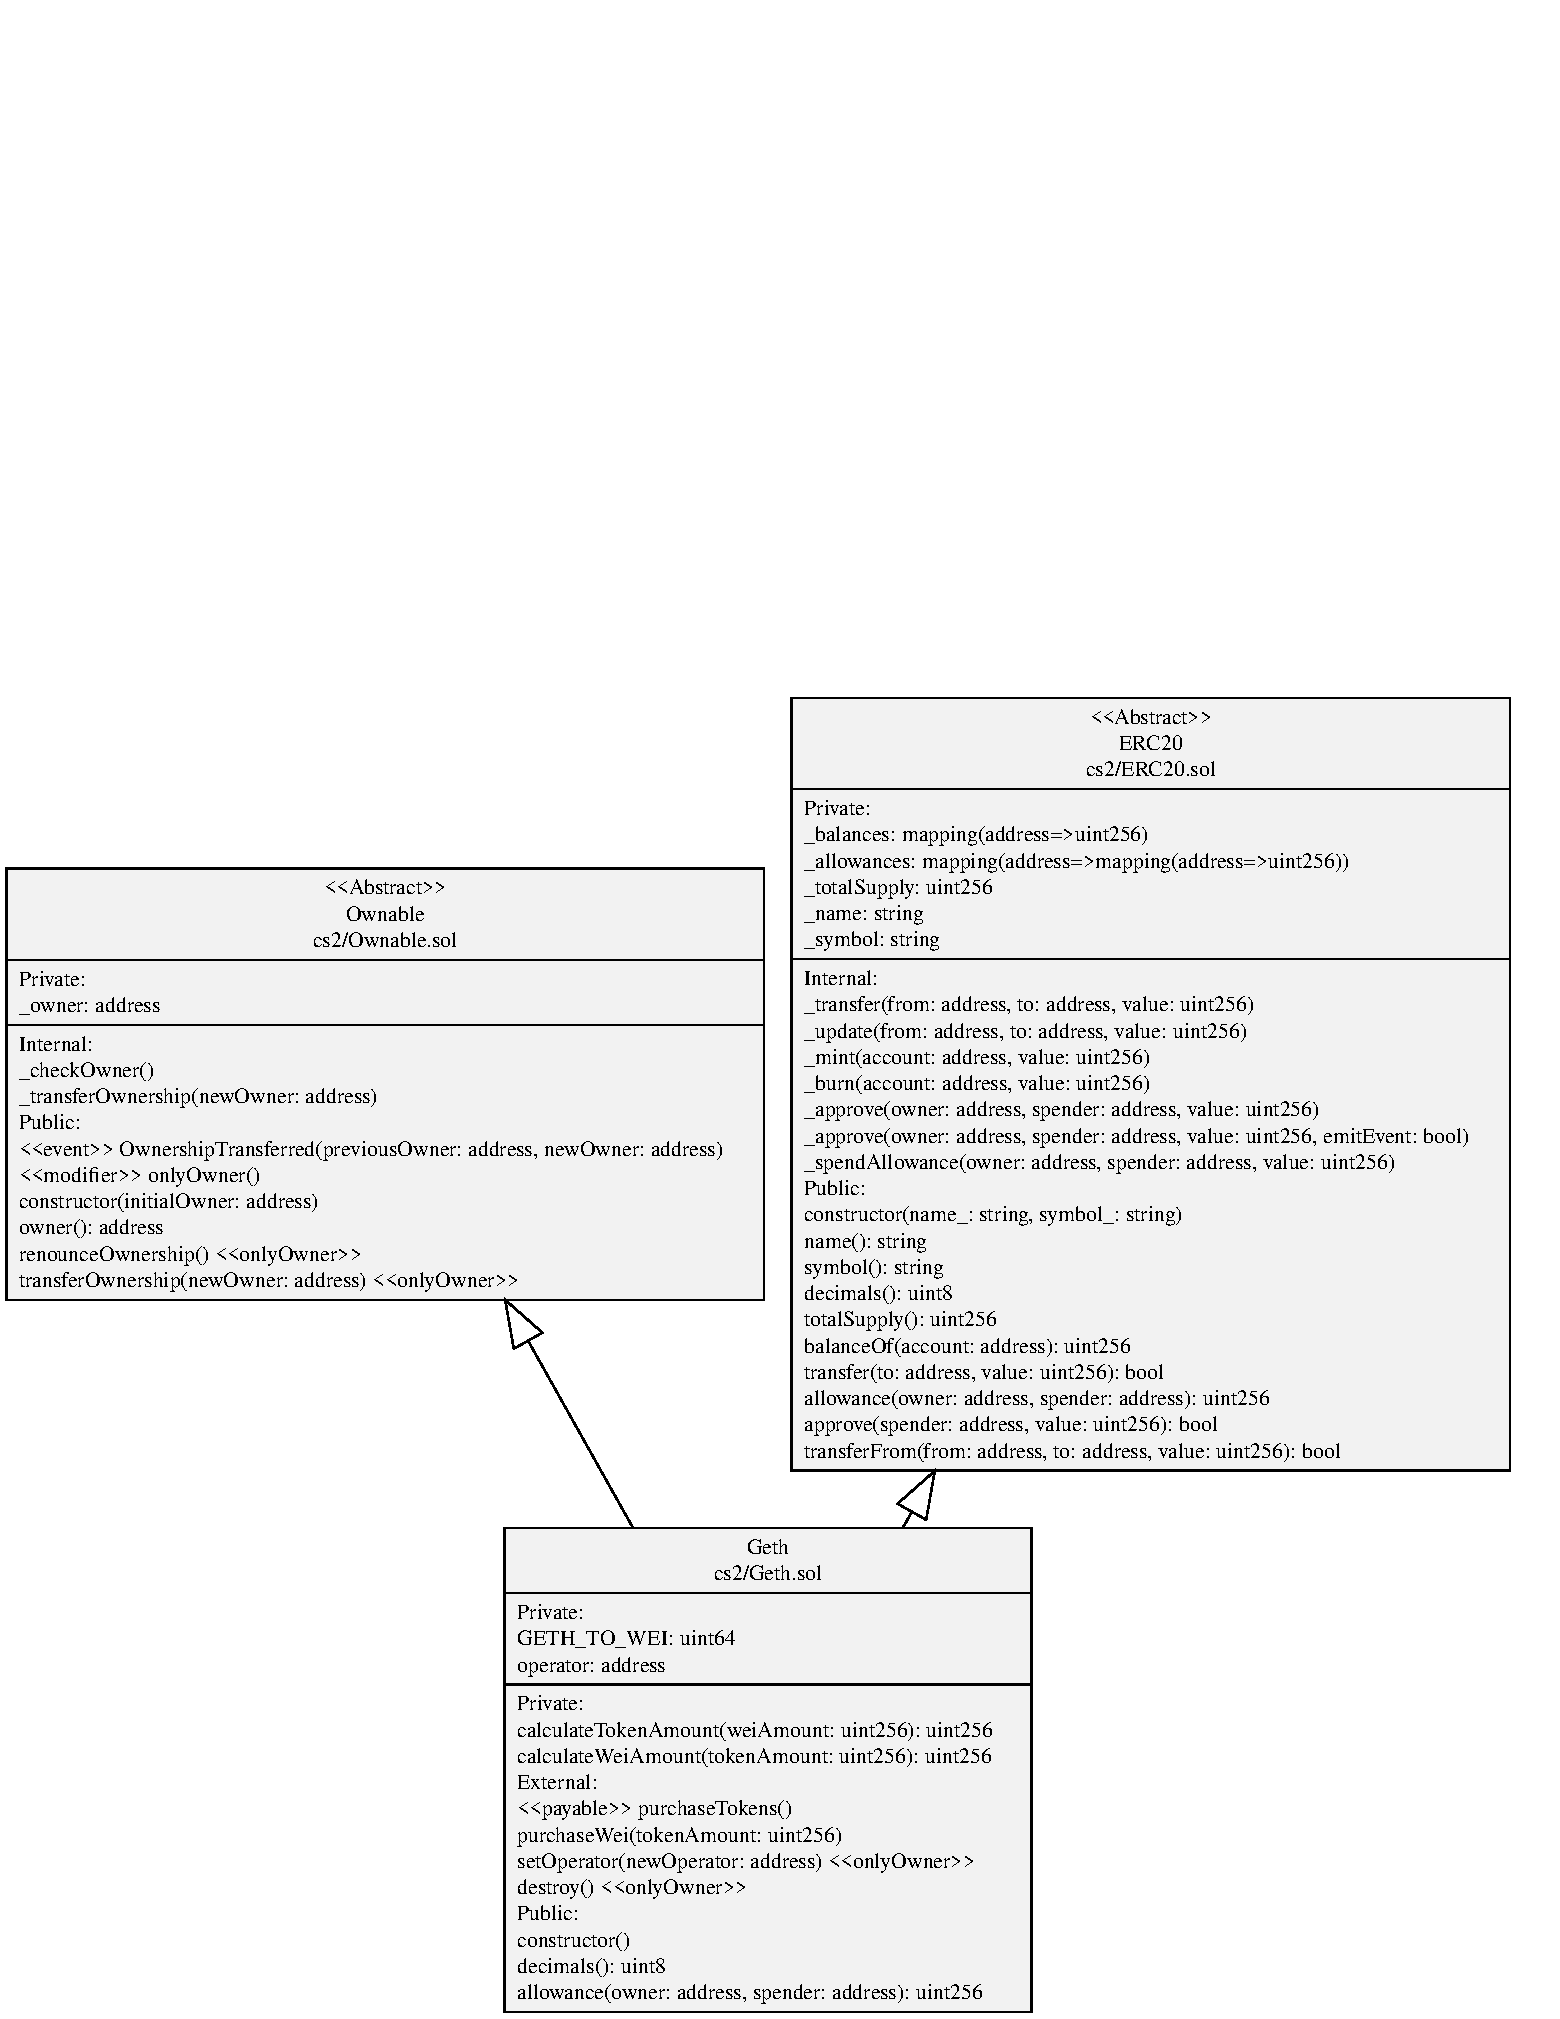
\includegraphics[scale=0.5]{figures/GETH.pdf}\\
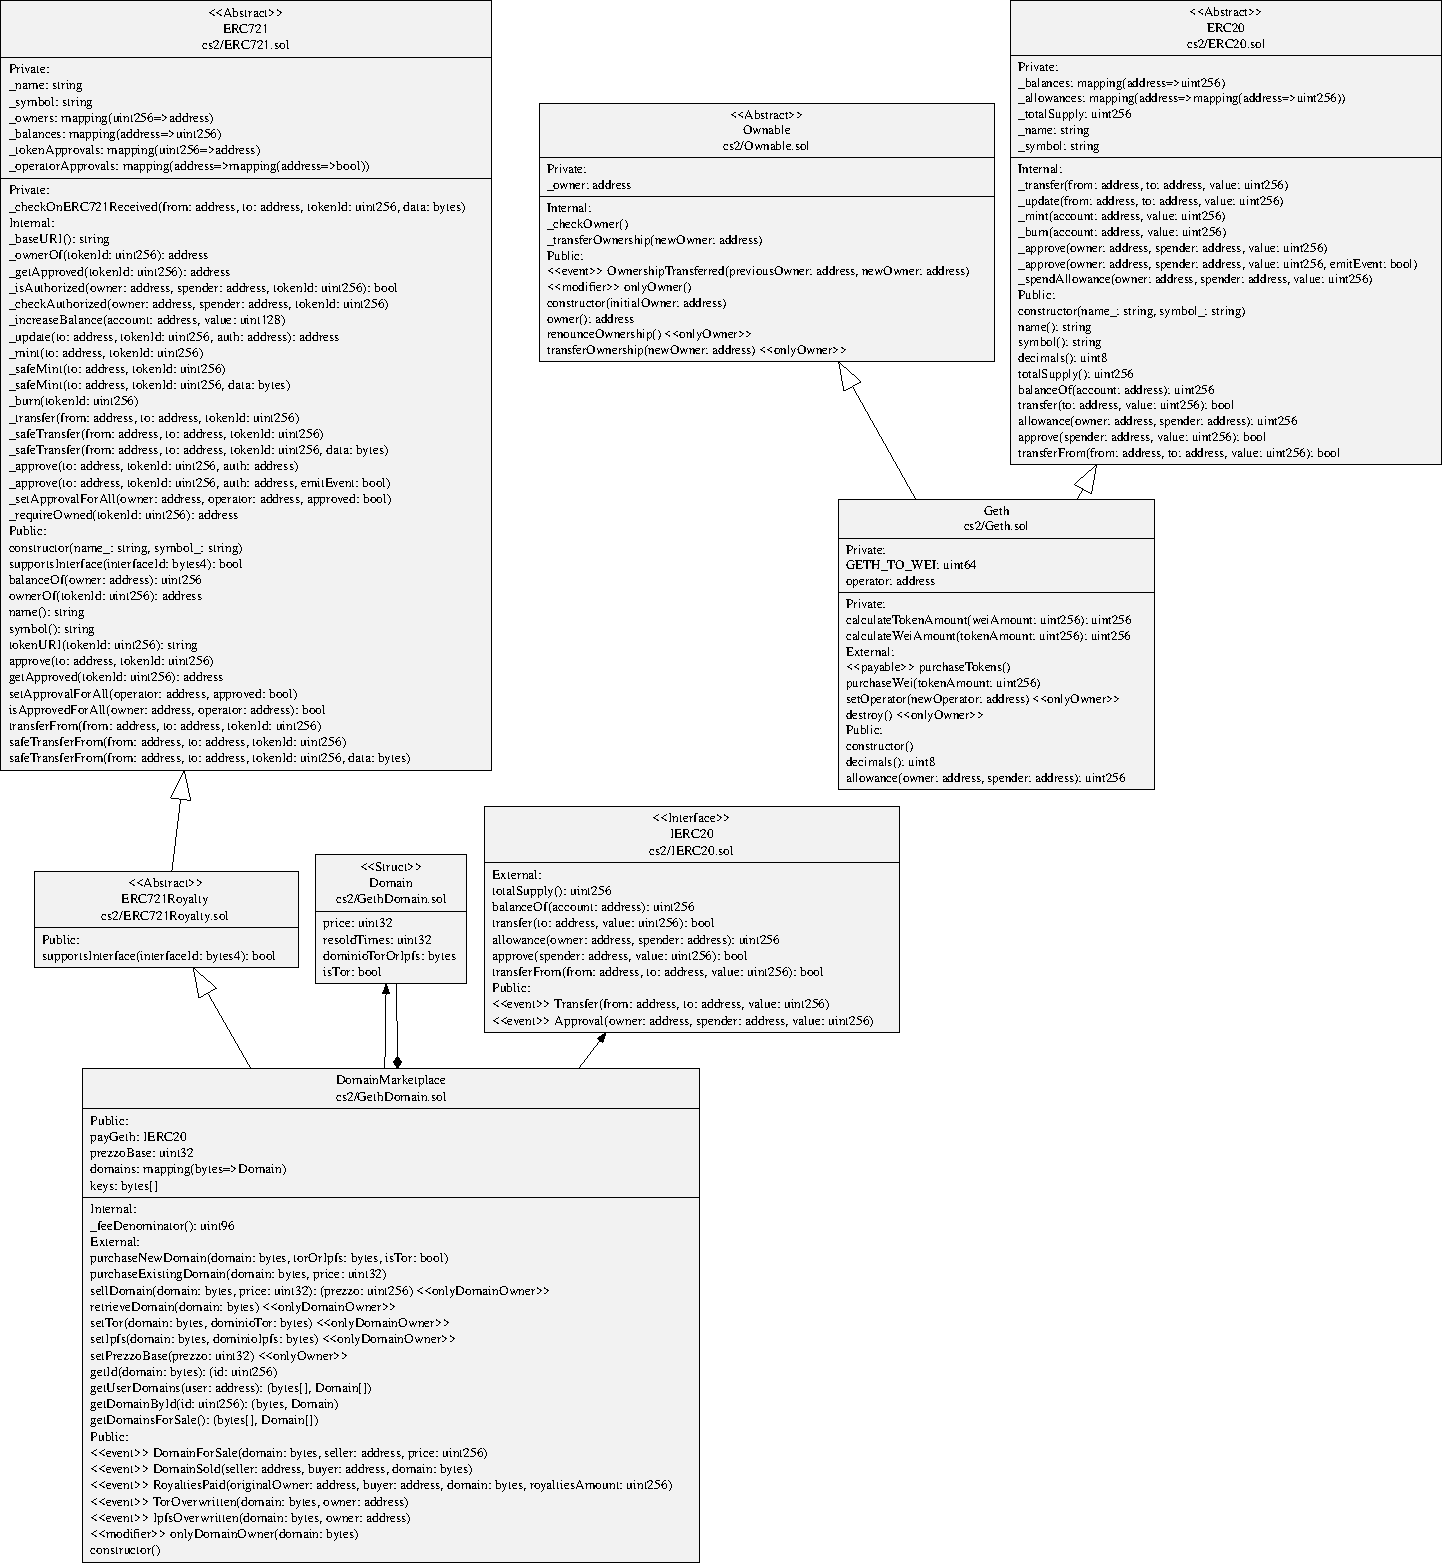
\includegraphics[scale=0.4]{figures/classDiag.pdf}

\subsection{Smart contracts}
The Geth Domain Dapp is based on fungible and non-fungible tokens.\\
The Geth contract manages the fungible token of the Dapp, used to buy a new or an existing domain.
The most important field of the smart contract is the operator, the address of another smart contract that will be allowed to spend geth from the balance of domain buyers.
The main functions are:
\begin{itemize}
    \item \texttt{purchaseTokens} is used to purchase Geth tokens with ETH, according to the established rate.
    \item \texttt{purchaseWei} is used to withdraw ETH with Geth tokens, according to the established rate
    \item \texttt{allowance} is used to stablish the amount that the operator can spend from the owner balance. This function has been overwritten to comply with the specification that states that the operator should be allowed to spend geth from the balance of domain buyers.
\end{itemize}
The DomainMarketplace contract regulates the NFT Domain name marketplace and registration. It follows ERC721 interface for interoperability and extends the abstract contract Ownable to manage operation security and ERC721Royalties to manage the royalties mechanism. Within the GethDomain.sol we define a struct that represents a Domain in our Dapp. The struct is composed of the following fields:
\begin{itemize}
    \item the \texttt{price} of the domain if it is for sale, or zero if not.
    \item the \texttt{resoldTimes} attribute that keeps how many times the domain is sold, to know when royalties should be payable.
    \item \texttt{pointedAddress} is a field containing a bytes pointer.
    \item \texttt{isTor} is a boolean to know which type of pointer is \texttt{pointedAddress}.
\end{itemize}
Within the GethDomain.sol we define some events to notify the clients to update the UI.
\begin{itemize}
    \item \texttt{DomainForSale} is emitted when a user sets his domain for sale by adding a price.
    \item \texttt{DomainSold} is emitted when a user buys an existing domain, previously settled for sale.
    \item \texttt{RoyaltiesPaid} is emitted to notify the creator of the domain that he received royalties by the sale. 
    \item \texttt{DomainPointerEdited} is emitted when an user overwrites the field \texttt{pointedAddress}.
\end{itemize}
In the smart contract is defined the \texttt{onlyDomainOwner} to check that the caller of a method is the owner of the domain concerned.
The DomainMarketplace has some fields such as:
\begin{itemize}
    \item \texttt{gethTokensContract}  is an instance of the erc20 used to pay the purchases.
    \item \texttt{newDomainPrice} used to keep a standard prize for purchasing a new domain in Geth.
    \item \texttt{domains} is the mapping of domains' information, given the bytes of an encoded name.
    \item \texttt{domainsKeys} is the list of all the domains' names, used to iterate over the mapping.
    \item \texttt{feeNumerator} is the numerator of the royalty fees fraction.
\end{itemize}
\newpage
The constructor of the smart contract is used to set the instance of the erc20 used to pay the purchases.
The main methods of the smart contract are:
\begin{itemize}
    \item \texttt{purchaseNewDomain} registers a new domain, given its name and the address it points to. The domain name is encoded as bytes, and then hashed to get the ID of the NFT. The domain is minted to the creator only after checking that the domain is not already registered and that the purchaser has enough Geth tokens to pay the registration fee. The price is set to 0 since it is not for sale and the geths paid are added to the contract balance. The domain is also set to point to the given address.
    \item \texttt{purchaseExistingDomain} is used to purchase an existing domain, given its name and price. The domain is transferred to the buyer, and the seller receives the price. The creator of the domain receives its royalties, if the domain has been resold. The function checks that the buyer is not the seller, that he must have enough Geth tokens to pay the price and the consistency between the price displayed in the UI and the actual cost. The domain name must already be for sale, otherwise the transaction will revert.
    \item \texttt{setNewDomainPrice}Set the price of a new domain, in Geth. This function can be called only by the contract owner thanks to the Ownable interface, because of its security implications.
\end{itemize}

Some functions have the \texttt{onlyDomainOwner} because they can be called only by the owner of the domain:
\begin{itemize}
    \item \texttt{sellDomain} puts a domain for sale, given its name and the price. The price must be greater than 0, otherwise the transaction will revert.
    \item \texttt{retrieveDomain} removes a domain from sale, given its name. The domain must be for sale, otherwise the transaction will revert.
    \item \texttt{setTor} and \texttt{setIPFS} edit a domain, given its name and the Tor or IPFS address it will point to.
\end{itemize}

It's worth noticing that the smart contracts Solidity source code is documented following the \textbf{NatSpec} format, following a standard for documentation.

\subsection{ERC1155 consideration}
We decided to use two smart contracts to manage our tokens instead of using only one implementing erc1155 because despite it allows grouping multiple transfers of different assets into a single transaction, thereby reducing the overall cost of operations, our functions don't transfer different assets from one user to another. So we preferred this approach to improve readability and reusability.

\subsection{Reentrancy attack consideration}
A reentrancy attack\cite{reentrancyAttack} occurs when a function makes an external call to another untrusted contract. Then the untrusted contract makes a recursive call back to the original function in an attempt to drain funds.
When the contract fails to update its state before sending funds, the attacker can continuously call the withdraw function to drain the contract’s funds. \texttt{PurchaseWei} function in geth.sol contract could be vulnerable to it but it's not, because it never makes a call to an external contract and most importantly, it follows the Check Effects Interactions pattern \cite{CEIPattern}. 

\subsection{Oracle considerations}
In our Dapp a domain can point to an address that may not exist. To avoid the user's mistakes, which means additional cost, we thought to use an oracle that checks the correctness of the pointer. After careful evaluation of our needs and the costs associated with using an external oracle, we have decided not to adopt this approach. Our decision is based on the fact that both the public key extracted by an onion address and the multi-base hash of IPFS address have their checksum. So in Tor is nearly impossible to make a mistake on a character that allows a match with another address. Instead in IPFS the hash is encoded through some base, so the decodification fails if some bytes don't match. In summary, our Dapp user is safe from this point of view, but an external user can still set an invalid TOR or IPFS address and that's on him.


\subsection{Data encoding and compression}
In the blockchain, we must save several types of string data, but reserving as few bytes as possible, in order to save costs.
In this section, we'll understand the different encoding strategies applied to achieve this result.

\subsubsection{Naive Domain Encoding}
The domain name is a string containing all lowercase ASCII letters from 'a' to 'z', ending in \texttt{.geth}.
Our goal is to shrink it as much as possible, in order to save the smallest amount of bytes possible on the blockchain.

The suffix can of course be removed since it's constant.

The first naive approach that comes into mind is to use 5 bits to encode each lowercase letter.
The calculation to reach this conclusion is simple:
\[ BitsPerChar = \lceil log_2({ord('z') - ord('a') + 1}) \rceil = 5 \]
Every 5 bits, a character is encoded so it's basically a task of reading 5 bits at a time from a Byte stream.

\subsubsection{Huffman Coding}
This coding, discussed theoretically in section \ref{sec:introduction_huffman}, it's practically applied to compress domains. Typically, Huffman guarantees the best compression possible, chunking the input stream every single byte, but it must also calculate the Huffman tree on the input to compress, and it must be stored. Storing this additional piece of data is absolutely counterproductive for our goal, but the intuition comes: the prior probability (or frequency) of a character appearing in the input text (i.e.: the domain name to compress) may be assumed to be very similar with respect to the average domain name already existing on the web.\\
We have collected data about the domain names registered on the standard web on 6 days, using a third-party service. More than 1.3 million domain names have been collected. They have finally been concatenated and the Huffman tree generation algorithm was run on that text.
The resulting tree is the one that is actually used for Gethdomains compression.\\
However, it works because is based on the strong assumption that the characters in the user input domain name follow the same probability distribution. This is not always the case, so in those cases, we fall back to the 5 bits encoding we have seen earlier.\\
The first bit (not byte) in the resulting byte array indicates the encoding used.

\subsubsection{Tor address encoding}
An Onion v3 address is basically a concatenation of the 32 bytes ECDSA public key of the hidden service, with its checksum and address version number.\cite{Tor_v3}\\
We can simply decode and extract the relevant 32 bytes, storing just them.\\
The onion address will be easily recalculated client-side by calculating the checksum and concatenating the various parts, encoding all of them as Base32 without padding.\\
This will make the original 62 characters long address, just 32 bytes.

\subsubsection{IPFS CID}
The CID (Content IDentifier) is a special string derived from the hash of the file. It exists in many forms, but since v0 is always convertible to v1, we will focus only on this one.\\
It is a concatenation of the following elements:\cite{IPFS_CID_v1_specification}
\begin{verbatim}
<cidv1> ::= <multibase-prefix>
            <multicodec-cidv1><multicodec-content-type>
            <multihash-content-address>
\end{verbatim}
\newpage
It is possible to process it as follows:
\begin{enumerate}
    \item Transform it from v0 to v1, if not already
    \item Decode the v1 string, according to the first character which indicates the Base that encodes the rest (according to the Multibase specification)
    \item Throw away the first decoded byte, which is always 1 in the v1 CID version
\end{enumerate}

While it's true that we have lost forever which was the original base that encoded the output or the version of the CID, these pieces of information are actually useless: re-encoding it in any base we want, in v1 version, will make it work just fine because of its interoperability.


\end{document}